\subsection{BÀI TẬP TRẮC NGHIỆM}
% \ind{PHẦN I.} \inden{Câu trắc nghiệm nhiều phương án lựa chọn. Học sinh trả lời từ câu 1 đến câu 12. Mỗi câu hỏi học sinh chỉ chọn một phương án.}\\
\TN
\setcounter{ex}{0}
\Opensolutionfile{ans}[ans/1D5-B1-1]
\begin{ex}%[1D3N1-1]
	Trong các mệnh đề dưới đây, mệnh đề nào \textbf{sai}?
	\choice
	{Nếu $\lim\limits_{n\to +\infty} u_n = +\infty$ và $\lim\limits_{n\to +\infty} v_n = a > 0$ thì $\lim\limits_{n\to +\infty}\left(u_n v_n\right)=+\infty$}
	{Nếu $\lim\limits_{n\to +\infty} u_n \neq 0$ và $\lim\limits_{n\to +\infty} v_n = \pm \infty$ thì $\lim\limits_{n\to +\infty}\left(\dfrac{u_n}{v_n}\right)=0$}
	{\True Nếu $\lim\limits_{n\to +\infty} u_n = a > 0$ và $\lim\limits_{n\to +\infty} v_n = 0$ thì $\lim\limits_{n\to +\infty}\left(\dfrac{u_n}{v_n}\right)=+\infty$}
	{Nếu $\lim\limits_{n\to +\infty} u_n = a < 0$ và $\lim\limits_{n\to +\infty} v_n = 0$ và $v_n > 0$ với mọi $n$ thì $\lim\limits_{n\to +\infty}\left(\dfrac{u_n}{v_n}\right)=-\infty$}
	\loigiai{
		Nếu $\lim\limits_{n\to +\infty} u_n = a > 0$ và $\lim\limits_{n\to +\infty} v_n = 0$ thì $\lim\limits_{n\to +\infty}\left(\dfrac{u_n}{v_n}\right)=+\infty$ là mệnh đề \textbf{sai} vì chưa rõ dấu của $v_n$ là dương hay âm.}
\end{ex}	

\begin{ex}%[1D3N1-1]
	Cho dãy số $\left( u_n\right)$ có $\lim\limits_{n\to +\infty} u_n=3$, dãy số  $\left( v_n\right)$ có $\lim\limits_{n\to +\infty} v_n=5$. Khi đó $\lim\limits_{n\to +\infty} \left(u_n v_n\right)$ bằng
	\choice
	{\True $15$}
	{$8$}
	{$5$}
	{$3$}
	\loigiai{
		Nếu $\lim\limits_{n\to +\infty} u_n= a$, $\lim\limits_{n\to +\infty} v_n=b$ thì $\lim\limits_{n\to +\infty} \left(u_n v_n\right)=a b$. Suy ra \[\lim\limits_{n\to +\infty} \left(u_n v_n\right)=3\cdot 5=15.\]}
\end{ex}	

\begin{ex}%[1D3N1-1]
	Cho $\lim\limits_{n\to +\infty} u_n=-3$, $\lim\limits_{n\to +\infty} v_n=2$. Khi đó $\lim\limits_{n\to +\infty} \left(u_n -v_n\right)$ bằng
	\choice
	{\True $-5$}
	{$-1$}
	{$2$}
	{$0$}
	\loigiai{
		Nếu $\lim\limits_{n\to +\infty} u_n= a$, $\lim\limits_{n\to +\infty} v_n=b$ thì $\lim\limits_{n\to +\infty} \left(u_n -v_n\right)=a-b$. Suy ra \[\lim\limits_{n\to +\infty} \left(u_n- v_n\right)=-3-2=-5.\]}
\end{ex}	

\begin{ex}%[1D3N1-1]
	Cho dãy số $\left( u_n\right)$ thỏa mãn $\lim\limits_{n\to +\infty} \left(u_n+3\right)=0$. Giá trị $\lim\limits_{n\to +\infty} u_n$ bằng
	\choice
	{$3$}
	{\True $-3$}
	{$2$}
	{$0$}
	\loigiai{
		Ta có  \[\lim\limits_{n\to +\infty} \left(u_n- 3\right)=0 \Leftrightarrow \lim\limits_{n\to +\infty} u_n=-3.\]}
\end{ex}

\begin{ex}%[1D3N1-1]
	Khẳng định nào sau đây là đúng?
	\choice
	{\True Ta nói dãy số $\left( u_n\right)$ có giới hạn là số $a$ khi $n\to +\infty$, nếu $\lim\limits_{n\to +\infty} \left(u_n-a\right)=0$}
	{Ta nói dãy số $\left( u_n\right)$ có giới hạn là $0$ khi $n$ dần tới vô cực, nếu $\left\vert u_n\right\vert$ có thể lớn hơn một số dương tùy ý, kể từ một số hạng nào đó trở đi}
	{Ta nói dãy số $\left( u_n\right)$ có giới hạn là $+\infty$ khi $n\to +\infty$, nếu $u_n$ có thể nhỏ hơn một số dương bất kì, kể từ một số hạng nào đó trở đi}
	{Ta nói dãy số $\left( u_n\right)$ có giới hạn là $-\infty$ khi $n\to +\infty$, nếu $u_n$ có thể lớn hơn một số dương bất kì, kể từ một số hạng nào đó trở đi}
	\loigiai{
		Theo định lí giới hạn hữu hạn của dãy số, dãy số $\left( u_n\right)$ có giới hạn là số $a$ khi $n\to +\infty$, nếu $\lim\limits_{n\to +\infty} \left(u_n-a\right)=0$.}
\end{ex}	

\begin{ex}%[1D3N1-1]
	Cho các dãy số $\left( u_n\right)$, $\left( v_n\right)$ và $\lim\limits_{n\to +\infty} u_n=a$, $\lim\limits_{n\to +\infty} v_n=+\infty$. Giá trị $\lim\limits_{n\to +\infty}\left( \dfrac{u_n}{v_n}\right)$ bằng
	\choice
	{$1$}
	{\True $0$}
	{$-\infty$}
	{$+\infty$}
	\loigiai{
		Dựa vào tính chất giới hạn dãy số, ta có nếu $\lim\limits_{n\to +\infty} u_n$ là một số hữu hạn và $\lim\limits_{n\to +\infty} v_n=+\infty$ thì $\lim\limits_{n\to +\infty}\left( \dfrac{u_n}{v_n}\right)=0$.}
\end{ex}

\begin{ex}%[1D3N1-1]
	Trong các khẳng định dưới đây, có bao nhiêu khẳng định đúng?
	\begin{enumerate}[(I)]
		\item $\lim\limits_{n\to +\infty} n^k=+\infty$ với $k$ nguyên dương.
		\item $\lim\limits_{n\to +\infty} q^n=+\infty$ nếu $\vert q\vert < 1$.
		\item $\lim\limits_{n\to +\infty} q^n=+\infty$ nếu $q > 1$.		
	\end{enumerate}
	\choice
	{$0$}
	{$1$}
	{$3$}
	{\True $2$}
	\loigiai{
		\begin{enumerate}[(I)]
			\item $\lim\limits_{n\to +\infty} n^k=+\infty$ với $k$ nguyên dương nên (I) là khẳng định đúng.
			\item $\lim\limits_{n\to +\infty} q^n=0$ nếu $\vert q\vert < 1$ nên (II) là khẳng định sai.
			\item $\lim\limits_{n\to +\infty} q^n=+\infty$ nếu $q > 1$ nên (III) là khẳng định đúng.	
		\end{enumerate}
		Vậy số khẳng định đúng là $2$.
	}
\end{ex}

\begin{ex}%[1D3N1-1]
	Phát biểu nào sau đây là \textbf{sai}?
	\choice
	{$\lim\limits_{n\to +\infty} u_n=c$ với $u_n=c$ là hằng số}
	{\True $\lim\limits_{n\to +\infty} q^n=0$ với  $\vert q\vert > 1$}
	{$\lim\limits_{n\to +\infty}\dfrac{1}{n}=0$}
	{$\lim\limits_{n\to +\infty}\dfrac{1}{n^k}=0$ với $k > 1$}
	\loigiai{
		Ta có $\lim\limits_{n\to +\infty} q^n=0$ với  $\vert q\vert < 1$.}
\end{ex}

\begin{ex}%[1D3N1-1]
	Dãy số nào sau đây có giới hạn bằng $0$?
	\choice
	{$\left(\dfrac{4}{e}\right)^n$}
	{$\left(\dfrac{5}{3}\right)^n$}
	{\True $\left(\dfrac{1}{3}\right)^n$}
	{$\left(-\dfrac{5}{3}\right)^n$}
	\loigiai{
		Vì $\left\vert \dfrac{1}{3}\right\vert =\dfrac{1}{3} < 1$ nên $\lim\limits_{n\to +\infty} \left(\dfrac{1}{3}\right)^n=0$.}
\end{ex}

\begin{ex}%[1D3N1-1]
	Giá trị $\lim\limits_{n\to +\infty}\dfrac{1}{n^2}$ bằng
	\choice
	{$+\infty$}
	{$1$}
	{$-\infty$}
	{\True $0$}
	\loigiai{
		Ta có $\lim\limits_{n\to +\infty}\dfrac{1}{n^k}=0$ với $k$ là số nguyên dương bất kì nên $\lim\limits_{n\to +\infty}\dfrac{1}{n^2}=0$.}
\end{ex}

\begin{ex}%[1D3N1-1]
	Dãy số nào có giới hạn khác $0$?
	\choice
	{$\left(\dfrac{4}{5}\right)^n$}
	{\True $2+\left(\dfrac{3}{5}\right)^n$}
	{$\dfrac{1}{2n}$}
	{$\left(\dfrac{1}{2}\right)^n$}
	\loigiai{
		Ta có $\lim\limits_{n\to +\infty}\left[2+\left(\dfrac{3}{5}\right)^n\right]=\lim\limits_{n\to +\infty} 2+\lim\limits_{n\to +\infty}\left(\dfrac{3}{5}\right)^n=2\neq 0$.}
\end{ex}

\begin{ex}%[1D3N1-1]
	Trong các khẳng định sau, khẳng định nào đúng?
	\choice
	{$\lim\limits_{n\to +\infty}\left(-\dfrac{1}{2}\right)^n=+\infty$}
	{$\lim\limits_{n\to +\infty} \left(-\dfrac{5}{n^3}\right)^n=-\infty$}
	{\True $\lim\limits_{n\to +\infty} \dfrac{1}{2} = \dfrac{1}{2}$}
	{$\lim\limits_{n\to +\infty}\left(\dfrac{4}{3}\right)^n=0$}
	\loigiai{
		Ta có $\lim\limits_{n\to +\infty} c=c$ với $c$ là hằng số nên  $\lim\limits_{n\to +\infty} \dfrac{1}{2} = \dfrac{1}{2}$.}
\end{ex}

\Closesolutionfile{ans}

% \ind{PHẦN II.} \inden{Câu trắc nghiệm đúng sai. Học sinh trả lời từ câu 1 đến câu 4. Trong mỗi ý a), b), c), d) ở mỗi câu, học sinh chọn đúng hoặc sai.}\\
\TNTF
\Opensolutionfile{ans}[ans/1D5-B1-2]
\setcounter{ex}{0}
\begin{ex}%[1D3H1-3]
	Cho hai dãy số $\left( u_n\right)$, $\left( v_n\right)$ với $u_n=\sqrt{9n^2+2n}-3n$, $v_n=-2+5n$.
	\choiceTF
	{\True $\lim\limits_{n\to +\infty}\dfrac{1}{v_n}=0$}
	{$\lim\limits_{n\to +\infty} v_n=-\infty$}
	{\True $\lim\limits_{n\to +\infty}\dfrac{u_n+3n}{v_n}=\dfrac{3}{5}$}
	{$\lim\limits_{n\to +\infty} u_n=0$}
	\loigiai{
		\begin{itemchoice}
			\itemch $\lim\limits_{n\to +\infty}\dfrac{1}{v_n}=\lim\limits_{n\to +\infty}\dfrac{1}{-2+5n}=\lim\limits_{n\to +\infty} \left(\dfrac{1}{n}\cdot \dfrac{1}{-\dfrac{2}{n}+5}\right)=0\cdot \dfrac{1}{5}=0$.
			\itemch Ta có \[\lim\limits_{n\to +\infty} v_n=\lim\limits_{n\to +\infty}\left(-2+5n\right)=\lim\limits_{n\to +\infty}\left[n\left(-\dfrac{2}{n}+5\right)\right].\]
			Mà $\lim\limits_{n\to +\infty} n=+\infty$ và $\lim\limits_{n\to +\infty}\left(-\dfrac{2}{n}+5\right)=5$ nên $\lim\limits_{n\to +\infty} v_n=+\infty$.
			\itemch $\lim\limits_{n\to +\infty}\dfrac{u_n+3n}{v_n}=\lim\limits_{n\to +\infty}\dfrac{\sqrt{9n^2+2n}}{-2+5n}=\lim\limits_{n\to +\infty}\dfrac{n\cdot\sqrt{9+\dfrac{2}{n^2}}}{n\cdot\left(-\dfrac{2}{n}+5\right)}=\lim\limits_{n\to +\infty} \dfrac{\sqrt{9+\dfrac{2}{n^2}}}{-\dfrac{2}{n}+5}=\dfrac{3}{5}$.
			\itemch Ta có 
			\begin{align*}
				\lim\limits_{n\to +\infty} u_n & =\lim\limits_{n\to +\infty} \left(\sqrt{9n^2+2n}-3n\right)
				\\ & =\lim\limits_{n\to +\infty}\dfrac{2n}{\sqrt{9n^2+2n}+3n}
				\\ & = \lim\limits_{n\to +\infty}\dfrac{2n}{n\cdot\left(\sqrt{9+\dfrac{2}{n^2}}+3\right)}
				\\ & =\lim\limits_{n\to +\infty}\dfrac{2}{\sqrt{9+\dfrac{2}{n^2}}+3}
				\\ &=\dfrac{2}{3+3}
				\\ &=\dfrac{1}{3}.
			\end{align*}
		\end{itemchoice}
	}
\end{ex}

\begin{ex}%[1D3H1-2]
	Cho hai dãy số $\left( u_n\right)$, $\left( v_n\right)$ với $u_n=4\cdot 3^n-7^{n+1}$, $v_n=7^n$.
	\choiceTF
	{\True $\lim\limits_{n\to +\infty}\dfrac{1}{v_n}=0$}
	{\True $\lim\limits_{n\to +\infty} v_n=+\infty$}
	{\True $\lim\limits_{n\to +\infty}\dfrac{u_n-v_n}{3u_n+2v_n}=\dfrac{8}{19}$}
	{$\lim\limits_{n\to +\infty} u_n=+\infty$}
	\loigiai{
		\begin{itemchoice}
			\itemch $\lim\limits_{n\to +\infty}\dfrac{1}{v_n}=\lim\limits_{n\to +\infty}\left(\dfrac{1}{7}\right)^n=0$.
			\itemch $\lim\limits_{n\to +\infty} v_n=\lim\limits_{n\to +\infty} 7^n=+\infty$.
			\itemch $ \lim\limits_{n\to +\infty}\dfrac{u_n-v_n}{3u_n+2v_n}=\lim\limits_{n\to +\infty}\dfrac{4\cdot 3^n-8\cdot 7^n}{12\cdot 3^n-19\cdot 7^n}=\lim\limits_{n\to +\infty}\dfrac{4\left(\dfrac{3}{7}\right)^n-8}{12\cdot \left(\dfrac{3}{7}\right)^n-19}=\dfrac{0-8}{0-19}=\dfrac{8}{19}$.
			\itemch Ta có \[ \lim\limits_{n\to +\infty} u_n=\lim\limits_{n\to +\infty}\left(4\cdot 3^n-7^{n+1}\right)=\lim\limits_{n\to +\infty} \left[ 7^n\left( 4\cdot \left(\dfrac{3}{7}\right)^n-7 \right) \right].\]
			Mà $\lim\limits_{n\to +\infty} 7^n=+\infty$, $\lim\limits_{n\to +\infty} \left[ 4\cdot \left(\dfrac{3}{7}\right)^n-7 \right] =-7 < 0 $ nên suy ra $\lim\limits_{n\to +\infty} u_n=-\infty$.
		\end{itemchoice}
	}
\end{ex}

\begin{ex}%[1D3H1-2]
	Cho hai dãy số $\left( u_n\right)$ và $\left( v_n\right)$ có $u_n=\dfrac{1}{n+1}$, $v_n=\dfrac{3}{n+3}$.
	\choiceTF
	{\True Ta nói dãy số $\left( u_n\right)$ có giới hạn là $0$ khi $n$ dần tới vô cực, vì $\vert u_n\vert$ có thể nhỏ hơn một số dương tùy ý, kể từ một số hạng nào đó trở đi}
	{\True $\lim\limits_{n\to +\infty} \left(v_n+1\right)=1$}
	{\True $\lim\limits_{n\to +\infty} \left(u_n-v_n\right)=0$}
	{\True $\lim\limits_{n\to +\infty} \dfrac{u_n}{v_n}=\dfrac{1}{3}$}
	\loigiai{
		\begin{itemchoice}
			\itemch Theo định nghĩa, ta có dãy số $\left( u_n\right)$ có giới hạn là $0$ khi $n$ dần tới vô cực, vì $\vert u_n\vert$ có thể nhỏ hơn một số dương tùy ý, kể từ một số hạng nào đó trở đi.
			\itemch $\lim\limits_{n\to +\infty} \left(v_n+1\right)=\lim\limits_{n\to +\infty} \left(\dfrac{3}{n+3}+1\right)=0+1=1$.
			\itemch Ta có 
			\begin{align*}
				\lim\limits_{n\to +\infty} \left(u_n-v_n\right) & =\lim\limits_{n\to +\infty} \left(\dfrac{1}{n+1}-\dfrac{3}{n+3}\right)
				\\ &= \lim\limits_{n\to +\infty} \dfrac{-2n}{(n+1)(n+3)}
				\\ &= \lim\limits_{n\to +\infty} \dfrac{-\dfrac{2}{n}}{\left(1+\dfrac{1}{n}\right)\left(1+\dfrac{3}{n}\right)}
				\\ &= 0.
			\end{align*}
			\itemch $\lim\limits_{n\to +\infty} \dfrac{u_n}{v_n}=\lim\limits_{n\to +\infty}\dfrac{\dfrac{1}{n+1}}{\dfrac{3}{n+3}}=\lim\limits_{n\to +\infty}\dfrac{n+3}{3(n+1)}=\lim\limits_{n\to +\infty}\dfrac{1+\dfrac{3}{n}}{3\left(1+\dfrac{1}{n}\right)}=\dfrac{1}{3}$.
		\end{itemchoice}
	}
\end{ex}

\begin{ex}%[1D3H1-4]
	Cho các dãy số $\left( u_n\right)$, $\left( v_n\right)$ có $\lim\limits_{n\to +\infty} u_n=-5$, $\lim\limits_{n\to +\infty} v_n=+\infty$. 
	\choiceTF
	{Ta nói dãy số $\left( u_n\right)$ có giới hạn là $-5$ khi $n$ dần tới vô cực, nếu $\lim\limits_{n\to +\infty} \left(u_n-5\right)=0$}
	{\True $\lim\limits_{n\to +\infty} \left(u_n+7\right)=2$}
	{$\lim\limits_{n\to +\infty} \left(u_n\cdot v_n\right)=+\infty$}
	{\True $\lim\limits_{n\to +\infty} \dfrac{u_n}{v_n}=0$}
	\loigiai{
		\begin{itemchoice}
			\itemch $\lim\limits_{n\to +\infty} u_n=-5$ nếu $\lim\limits_{n\to +\infty} \left(u_n-5\right)=-10$.
			\itemch $\lim\limits_{n\to +\infty} \left(u_n+7\right)=\lim\limits_{n\to +\infty} u_n+\lim\limits_{n\to +\infty} 7=-5+7=2$.
			\itemch Do $\lim\limits_{n\to +\infty} u_n=-5<0$ và $\lim\limits_{n\to +\infty} v_n=+\infty$ nên $\lim\limits_{n\to +\infty} \left(u_n\cdot v_n\right)=-\infty$.
			\itemch Do $\lim\limits_{n\to +\infty} u_n=-5$ và $\lim\limits_{n\to +\infty} v_n=+\infty$ nên $\lim\limits_{n\to +\infty} \dfrac{u_n}{v_n}=0$.
		\end{itemchoice}
	}
\end{ex}
\Closesolutionfile{ans}

% \ind{PHẦN III.} \inden{Câu trắc nghiệm trả lời ngắn. Học sinh trả lời từ câu 1 đến câu 6.}\\
\TNSA
\Opensolutionfile{ans}[ans/1D5-B1-3]
\setcounter{ex}{0}
\begin{ex}%[1D3H1-3]
	Tính tích các giá trị nguyên của $a$ thỏa mãn $\lim\limits_{n\to +\infty}\left(\sqrt{n^2-8n}-n+a^2\right)=0$.\\
	\shortans[oly]{$-4$}
	\loigiai{
		Ta có 
		\begin{align*}
			\lim\limits_{n\to +\infty}\left(\sqrt{n^2-8n}-n+a^2\right)&=\lim\limits_{n\to +\infty}\left(\dfrac{n^2-8n-n^2}{\sqrt{n^2-8n}+n}+a^2\right)
			\\ & = \lim\limits_{n\to +\infty}\left(\dfrac{-8n}{n\sqrt{1-\dfrac{8}{n}}+n}+a^2\right)
			\\ & = \lim\limits_{n\to +\infty}\left(\dfrac{-8}{\sqrt{1-\dfrac{8}{n}}+1}+a^2\right)
			\\ & = -4+a^2.
		\end{align*}
		Để $\lim\limits_{n\to +\infty}\left(\sqrt{n^2-8n}-n+a^2\right)=0$ thì $-4+a^2=0$ hay $a=\pm 2$. 
		\\ Suy ra tích các giá trị nguyên của $a$ là $-4$.
	}
\end{ex}

\begin{ex}%[1D3V1-6]
	Từ độ cao $55{,}8$ m của tháp nghiêng Pisa nước Ý, người ta thả một quả bóng cao su chạm xuống đất (như hình vẽ). Giả sử mỗi lần chạm đất quả bóng lại nảy lên độ cao bằng $\dfrac{1}{10}$ độ cao mà quả bóng đạt được trước đó. Tính tổng độ dài quãng đường di chuyển của quả bóng tính từ lúc thả ban đầu cho đến khi quả bóng đó dừng hẳn trên mặt đất.
	\definecolor{lightcornflowerblue}{rgb}{0.6, 0.81, 0.93}
	\definecolor{cadmiumgreen}{rgb}{0.0, 0.42, 0.24}
	\definecolor{trueblue}{rgb}{0.0, 0.45, 0.81}
	\definecolor{tumbleweed}{rgb}{0.87, 0.67, 0.53}%màu cát
	
	\begin{center}
		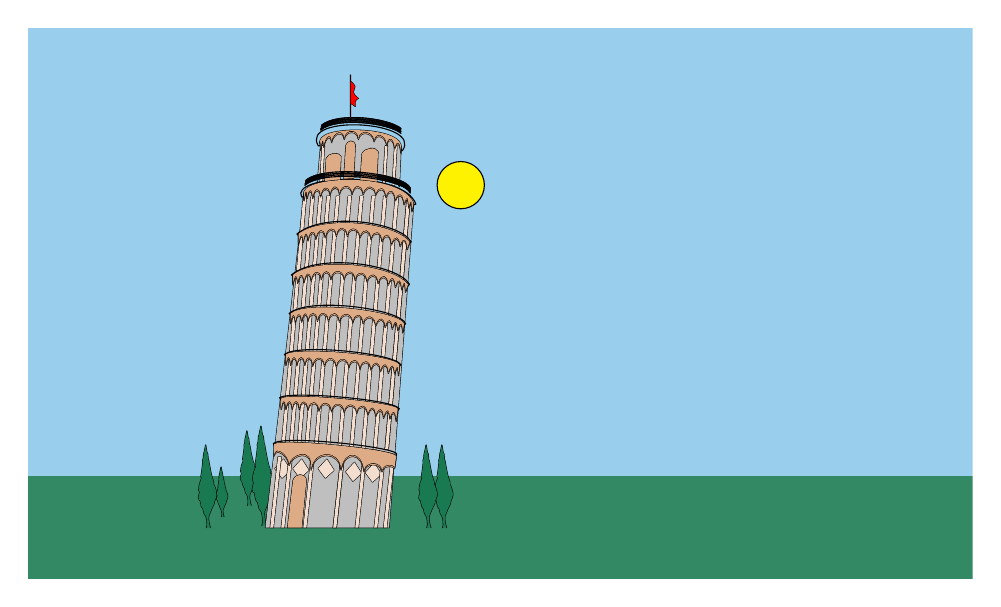
\begin{tikzpicture}[line join=round, line cap=round,scale=1,transform shape]
			\clip (-4,-3.5) rectangle (8,3.5);
			
			\tikzset{thap/.pic={%Xây từ dưới lên
					\def\T{ 
						(-.88,-1.78)%1
						..controls +(40:.17) and +(120:.1) ..  (.686,-1.91)--(.68,-1.94)
						..controls +(120:.1) and +(40:.12) ..  (-.87,-1.81)
						--cycle
						
						(-.8,-1.2)%2
						..controls +(40:.14) and +(120:.14) ..  (.72,-1.34)--(.7,-1.36)
						..controls +(120:.1) and +(40:.12) ..  (-.78,-1.23)
						--cycle
						
						(-.74,-.65)%3
						..controls +(40:.22) and +(120:.17) ..  (.74,-.78)--(.72,-.8)
						..controls +(120:.15) and +(40:.15) ..  (-.72,-.67)
						--cycle
						
						(-.68,-.13)%4
						..controls +(40:.34) and +(110:.2) ..  (.8,-.26)--(.78,-.28)
						..controls +(110:.17) and +(40:.27) ..  (-.66,-.15)
						--cycle
						
						(-.65,.36)%5
						..controls +(40:.44) and +(120:.3) ..  (.85,.24)--(.83,.22)
						..controls +(130:.35) and +(40:.35) ..  (-.63,.34)
						--cycle
						
						(-.58,.88)%6
						..controls +(40:.44) and +(120:.3) ..  (.87,.78)--(.85,.76)
						..controls +(130:.35) and +(40:.35) ..  (-.56,.86)
						--cycle
						
						(-.52,1.35)%7
						..controls +(120:.32) and +(110:.47) ..  (.93,1.26)--(.9,1.25)
						..controls +(110:.43) and +(110:.27) ..  (-.49,1.35)
						--cycle
						
						(-.31,2)%8
						..controls +(120:.47) and +(55:.46) ..  (.76,1.94)--(.74,1.94)
						..controls +(75:.31) and +(115:.28) ..  (-.28,2)
						--cycle
						
						(-.48,1.5)
						..controls +(40:.33) and +(110:.2) ..  (.86,1.4)
						(-.476,1.52)
						..controls +(40:.33) and +(110:.2) ..  (.86,1.42)
						(-.472,1.54)
						..controls +(40:.33) and +(110:.2) ..  (.86,1.44)
						(-.468,1.56)
						..controls +(40:.33) and +(110:.2) ..  (.86,1.46)
						
						(-.28,2.2)
						..controls +(40:.27) and +(140:.2) ..  (.74,2.16)
						(-.276,2.22)
						..controls +(40:.27) and +(140:.2) ..  (.74,2.18)
						(-.272,2.24)
						..controls +(40:.27) and +(140:.2) ..  (.74,2.2)
						(-.268,2.26)
						..controls +(40:.27) and +(140:.2) ..  (.74,2.22)
						;}
					\draw \T;
					%\fill[tumbleweed] \T;
			}}
			
			\tikzset{rao/.pic={%Rào
					\def\R{ 
						(-.48,1.5)
						..controls +(40:.33) and +(110:.2) ..  (.86,1.4)
						(-.476,1.52)
						..controls +(40:.33) and +(110:.2) ..  (.86,1.42)
						(-.472,1.54)
						..controls +(40:.33) and +(110:.2) ..  (.86,1.44)
						(-.468,1.56)
						..controls +(40:.33) and +(110:.2) ..  (.86,1.46)
						(-.28,2.2)
						..controls +(40:.27) and +(140:.2) ..  (.74,2.16)
						(-.276,2.22)
						..controls +(40:.27) and +(140:.2) ..  (.74,2.18)
						(-.272,2.24)
						..controls +(40:.27) and +(140:.2) ..  (.74,2.2)
						(-.268,2.26)
						..controls +(40:.27) and +(140:.2) ..  (.74,2.22)
						;}
					\draw \R;
					%\fill[tumbleweed] \R;
			}}
			
			\tikzset{co/.pic={%Cờ
					\def\C{ 
						(0.1,2.3)--(.1,2.9)
						(.1,2.82)
						..controls +(-40:.2) and +(140:.22) ..  (.2,2.6)
						..controls +(-60:0) and +(100:.1) ..(.16,2.5)
						..controls +(140:.1) and +(-30:0) ..  (.1,2.53)--cycle
						;}
					\draw \C;
					\fill[red] \C;
			}}
			
			\tikzset{cong0/.pic={%Đường cong trệt
					\def\D0{ 
						(.68,-1.96)
						..controls +(120:.1) and +(40:.12) ..  (-.87,-1.81)--
						(-.87,-1.94)
						..controls +(80:.12) and +(95:0.12) ..  (-.68,-2.06)
						..controls +(80:.12) and +(85:0.3) ..  (-.4,-2.12)
						..controls +(80:.25) and +(95:0.25) ..  (-.02,-2.12)
						..controls +(80:.25) and +(95:0.25) ..  (.27,-2.14)
						..controls +(80:.12) and +(95:0.12) ..  (.5,-2.14)
						..controls +(70:.12) and +(95:0.02) ..  (.66,-2.1)--cycle
						;}
					\draw \D0;
					\fill[tumbleweed] \D0;
			}}
			
			\tikzset{cong1/.pic={%Đường cong 1
					\def\D1{ 
						(.7,-1.36)
						..controls +(120:.1) and +(40:.12) ..  (-.78,-1.23)--
						(-.78,-1.35)
						..controls +(80:.12) and +(95:0.12) ..  (-.72,-1.35)
						..controls +(80:.12) and +(95:0.12) ..  (-.64,-1.35)
						..controls +(80:.12) and +(95:0.12) ..  (-.55,-1.35)
						..controls +(80:.12) and +(95:0.12) ..  (-.44,-1.36)
						..controls +(80:.12) and +(95:0.12) ..  (-.3,-1.37)
						..controls +(80:.12) and +(95:0.12) ..  (-.14,-1.38)
						..controls +(80:.12) and +(95:0.12) ..  (0.02,-1.39)
						..controls +(80:.12) and +(95:0.12) ..  (0.18,-1.4)
						..controls +(80:.12) and +(95:0.12) ..  (0.32,-1.42)
						..controls +(70:.12) and +(95:0.12) ..  (0.42,-1.44)
						..controls +(70:.12) and +(95:0.12) ..  (0.52,-1.46)
						..controls +(70:.12) and +(95:0.12) ..  (0.6,-1.47)
						..controls +(70:.12) and +(95:0.12) ..  (0.68,-1.5)--cycle
						;}
					\draw \D1;
					\fill[tumbleweed] \D1;
			}}
			
			\tikzset{cong2/.pic={%Đường cong 2
					\def\D2{ 
						(.72,-.8)
						..controls +(120:.15) and +(40:.15) ..  (-.72,-.67)--
						(-.72,-.79)
						..controls +(80:.12) and +(95:0.12) ..  (-.66,-.79)
						..controls +(80:.12) and +(95:0.12) ..  (-.58,-.79)
						..controls +(80:.12) and +(95:0.12) ..  (-.48,-.79)
						..controls +(80:.12) and +(95:0.12) ..  (-.38,-.8)
						..controls +(80:.12) and +(95:0.12) ..  (-.23,-.8)
						..controls +(80:.12) and +(95:0.12) ..  (-0.08,-.81)
						..controls +(80:.12) and +(95:0.12) ..  (0.08,-.82)
						..controls +(80:.12) and +(95:0.12) ..  (0.22,-.84)
						..controls +(80:.12) and +(95:0.12) ..  (0.36,-.85)
						..controls +(70:.12) and +(95:0.12) ..  (0.48,-.87)
						..controls +(70:.12) and +(95:0.12) ..  (0.58,-.89)
						..controls +(70:.12) and +(95:0.12) ..  (0.66,-.9)
						..controls +(70:.12) and +(95:0.12) ..  (0.71,-.92)--cycle
						;}
					\draw \D2;
					\fill[tumbleweed] \D2;
			}}
			
			\tikzset{cong3/.pic={%Đường cong 3
					\def\D3{ 
						(.78,-.28)
						..controls +(110:.17) and +(40:.27) ..  (-.66,-.15)--
						(-.66,-.26)
						..controls +(80:.12) and +(95:0.12) ..  (-.6,-.25)
						..controls +(80:.12) and +(95:0.12) ..  (-.52,-.24)
						..controls +(80:.12) and +(95:0.12) ..  (-.44,-.23)
						..controls +(80:.12) and +(95:0.12) ..  (-.32,-.23)
						..controls +(80:.12) and +(95:0.12) ..  (-.18,-.23)
						..controls +(80:.12) and +(95:0.12) ..  (-.04,-.24)
						..controls +(80:.12) and +(95:0.12) ..  (0.13,-.25)
						..controls +(80:.12) and +(95:0.12) ..  (0.26,-.26)
						..controls +(70:.12) and +(95:0.12) ..  (0.42,-.29)
						..controls +(70:.12) and +(95:0.12) ..  (0.54,-.31)
						..controls +(70:.12) and +(95:0.12) ..  (0.63,-.33)
						..controls +(70:.12) and +(95:0.12) ..  (0.7,-.35)
						..controls +(70:.12) and +(95:0.12) ..  (0.765,-.38)--cycle
						;}
					\draw \D3;
					\fill[tumbleweed] \D3;
			}}
			
			\tikzset{cong4/.pic={%Đường cong 4
					\def\D4{ 
						(.83,.22)
						..controls +(130:.35) and +(40:.35) ..  (-.63,.34)--
						(-.63,.23)
						..controls +(80:.12) and +(95:0.12) ..  (-.57,.25)
						..controls +(80:.12) and +(95:0.12) ..  (-.49,.26)
						..controls +(80:.12) and +(95:0.12) ..  (-.4,.28)
						..controls +(80:.12) and +(95:0.12) ..  (-.27,.3)
						..controls +(80:.12) and +(95:0.12) ..  (-.15,.3)
						..controls +(80:.12) and +(95:0.12) ..  (0.02,.3)
						..controls +(80:.12) and +(95:0.12) ..  (0.16,.29)
						..controls +(80:.12) and +(95:0.12) ..  (0.31,.27)
						..controls +(70:.12) and +(95:0.12) ..  (0.45,.25)
						..controls +(70:.12) and +(95:0.12) ..  (0.58,.23)
						..controls +(70:.12) and +(95:0.12) ..  (0.67,.2)
						..controls +(70:.12) and +(95:0.12) ..  (0.75,.17)
						..controls +(70:.12) and +(95:0.12) ..  (0.8,.14)--cycle
						;}
					\draw \D4;
					\fill[tumbleweed] \D4;
			}}
			
			\tikzset{cong5/.pic={%Đường cong 5
					\def\D5{ 
						(.85,.76)
						..controls +(130:.35) and +(40:.35) ..  (-.56,.86)--
						(-.56,.74)
						..controls +(80:.12) and +(95:0.12) ..  (-.5,.77)
						..controls +(80:.12) and +(95:0.12) ..  (-.44,.79)
						..controls +(80:.12) and +(95:0.12) ..  (-.34,.81)
						..controls +(80:.12) and +(95:0.12) ..  (-.22,.83)
						..controls +(80:.12) and +(95:0.12) ..  (-0.08,.85)
						..controls +(80:.12) and +(95:0.12) ..  (0.06,.85)
						..controls +(80:.12) and +(95:0.12) ..  (0.22,.83)
						..controls +(70:.12) and +(95:0.12) ..  (0.36,.81)
						..controls +(70:.12) and +(95:0.12) ..  (0.5,.78)
						..controls +(70:.12) and +(95:0.12) ..  (0.62,.74)
						..controls +(70:.12) and +(95:0.12) ..  (0.73,.72)
						..controls +(70:.12) and +(95:0.12) ..  (0.82,.68)--cycle
						;}
					\draw \D5;
					\fill[tumbleweed] \D5;
			}}
			
			\tikzset{cong6/.pic={%Đường cong 6
					\def\D6{ 
						(.9,1.25)
						..controls +(110:.43) and +(110:.27) ..  (-.49,1.35)--
						(-.49,1.3)
						..controls +(80:.12) and +(95:0.12) ..  (-.45,1.33)
						..controls +(80:.12) and +(95:0.12) ..  (-.38,1.33)
						..controls +(80:.12) and +(95:0.12) ..  (-.28,1.35)
						..controls +(80:.12) and +(95:0.12) ..  (-.16,1.37)
						..controls +(80:.12) and +(95:0.12) ..  (-0.04,1.38)
						..controls +(80:.12) and +(95:0.12) ..  (0.12,1.38)
						..controls +(80:.12) and +(95:0.12) ..  (0.26,1.38)
						..controls +(70:.12) and +(95:0.12) ..  (0.42,1.37)
						..controls +(70:.12) and +(95:0.12) ..  (0.55,1.34)
						..controls +(70:.12) and +(95:0.12) ..  (0.67,1.3)
						..controls +(70:.12) and +(95:0.12) ..  (0.78,1.25)
						..controls +(70:.12) and +(95:0.12) ..  (0.84,1.21)
						..controls +(70:.12) and +(95:0.12) ..  (0.88,1.16)--cycle
						;}
					\draw \D6;
					\fill[tumbleweed] \D6;
			}}
			
			\tikzset{cong7/.pic={%Đường cong 7
					\def\D7{ 
						(.74,1.94)
						..controls +(75:.31) and +(115:.28) ..  (-.28,2)--
						(-.28,1.94)
						..controls +(80:.12) and +(95:0.12) ..  (-.24,1.98)
						..controls +(80:.12) and +(95:0.12) ..  (-.14,2.04)
						..controls +(80:.12) and +(95:0.12) ..  (0.02,2.08)
						..controls +(80:.12) and +(95:0.12) ..  (0.2,2.08)
						..controls +(80:.12) and +(95:0.12) ..  (0.4,2.05)
						..controls +(80:.12) and +(95:0.12) ..  (0.56,2)
						..controls +(80:.12) and +(95:0.12) ..  (0.66,1.96)
						..controls +(70:.12) and +(95:0.12) ..  (0.74,1.9)--cycle
						;}
					\draw \D7;
					\fill[tumbleweed] \D7;
			}}
			
			\tikzset{cua/.pic={%Cửa
					\def\W{ 
						(-.7,-2.85)--(-.63,-2.25)
						..controls +(70:.1) and +(100:.1) ..  (-.46,-2.25)--(-.52,-2.85)
						--cycle
						;}
					\draw \W;
					\fill[tumbleweed] \W;
			}}
			
			\tikzset{vien/.pic={%viền ngoài
					\def\V{ 
						(.9,1.25)
						..controls +(110:.43) and +(110:.27) ..  (-.49,1.35)--(-.98,-2.85)--(.59,-2.85)--cycle
						
						(.74,1.94)
						..controls +(75:.31) and +(115:.28) ..  (-.28,2)--(-.32,1.54)
						..controls +(115:.2) and +(75:.13) ..  (.72,1.48)--cycle
						;}
					\draw \V;
					\fill[gray!50!] \V;
			}}
			
			\tikzset{soc/.pic={%Thanh sọc
					\def\S{ 
						(.82,1.36)--(.54,-1.85)--(.58,-1.85)--(.86,1.36)
						--cycle
						;}
					\draw \S;
					\fill[tumbleweed!40!] \S;
			}}
			
			\tikzset{soc2/.pic={%Thanh sọc lớn
					\def\S{ 
						(.54,-1.95)--(.44,-2.85)--(.48,-2.85)--(.58,-1.95)
						--cycle
						;}
					\draw \S;
					\fill[tumbleweed!40!] \S;
			}}
			
			\tikzset{soc3/.pic={%Thanh sọc
					\def\S{ 
						(.54,2)--(.57,2)--(.54,1.5)--(.51,1.5)
						--cycle
						(.66,2)--(.69,2)--(.66,1.5)--(.63,1.5)
						--cycle
						(-.26,2)--(-.23,2)--(-.26,1.5)--(-.29,1.5)
						--cycle
						;}
					\draw \S;
					\fill[tumbleweed!40!] \S;
			}}
			
			\tikzset{thoi/.pic={%Hình thoi
					\def\T{ 
						(0.15,-1.98)--(.24,-2.12)--(0.13,-2.22)--(0.04,-2.1)
						--cycle
						;}
					\draw \T;
					\fill[tumbleweed!40!] \T;
			}}
			
			\tikzset{cay/.pic={%Cây
					\def\T{ 
						(-1.73,-2.85)
						..controls +(40:.03) and +(40:.01) ..  (-1.74,-2.7)
						..controls +(140:.04) and +(60:.02) ..  (-1.78,-2.6)
						..controls +(140:.04) and +(60:.02) ..  (-1.8,-2.55)
						..controls +(100:.03) and +(70:.02) ..  (-1.82,-2.5)
						..controls +(140:.04) and +(60:.02) ..  (-1.815,-2.4)
						..controls +(140:.04) and +(60:.02) ..  (-1.818,-2.3)
						..controls +(85:.03) and +(-30:.03) ..  (-1.8,-2.2)
						..controls +(80:.04) and +(50:.02) ..  (-1.78,-2)
						..controls +(60:.04) and +(120:.02) ..  (-1.76,-1.9)
						..controls +(80:.03) and +(-100:.02) ..  (-1.74,-1.8)
						..controls +(80:.01) and +(-100:.02) ..  (-1.72,-1.9)
						..controls +(60:.02) and +(-120:.02) ..  (-1.7,-2)
						..controls +(-80:.02) and +(110:.03) ..  (-1.66,-2.2)
						..controls +(-100:.02) and +(60:.03) ..  (-1.64,-2.3)
						..controls +(-30:.02) and +(70:.02) ..  (-1.6,-2.44)
						..controls +(-100:.02) and +(70:.02) ..  (-1.63,-2.52)
						..controls +(-60:.02) and +(70:.01) ..  (-1.66,-2.6)
						..controls +(60:.01) and +(70:.02) ..  (-1.7,-2.7)
						..controls +(-120:.02) and +(120:.03) ..  (-1.68,-2.85)
						;}
					\draw \T;
					\fill[cadmiumgreen!90!] \T;
			}}
			\fill[cadmiumgreen!80!] (-4,-3.5) rectangle (8,-2.2);
			\fill[lightcornflowerblue] (-4,3.5) rectangle (8,-2.2);
			\path 
			(0,0)pic[scale=1]{cay}(.35,0)pic[scale=.9]{cay}(1.05,0.6)pic[scale=1.2]{cay}(-.5,-1)pic[scale=.6]{cay}
			(3,0)pic[scale=1]{cay}(2.8,0)pic[scale=1]{cay}
			(0,0)pic[scale=1]{vien}
			(0,0)pic[scale=1]{soc} (0,0)pic[scale=1]{soc}(-.15,0)pic[scale=1]{soc}(-.3,0)pic[scale=1]{soc}(-.45,0)pic[scale=1]{soc}(-.6,0)pic[scale=1]{soc}(-.75,0)pic[scale=1]{soc}(-.9,0)pic[scale=1]{soc}(-1.02,0)pic[scale=1]{soc}(-1.12,0)pic[scale=1]{soc}(-1.22,0)pic[scale=1]{soc}(-1.32,0)pic[scale=1]{soc}
			
			(0,0)pic[scale=1]{soc3}
			(0,0)pic[scale=1]{thap}(0,0)pic[scale=1]{co}
			(.4,3.6)pic[scale=.7,rotate=3]{cua}
			(.8,3.6)pic[scale=1.2,rotate=7,yscale=.6]{cua}
			(.3,3.4)pic[scale=1.1,rotate=7,yscale=.6]{cua}
			(0,-.04)pic[scale=1]{thoi}(0.25,-.05)pic[scale=1]{thoi}(-0.35,0)pic[scale=1]{thoi}(-.67,0)pic[scale=1]{thoi}(-.9,0)pic[scale=1]{thoi}
			(-1.22,0)pic[scale=1]{soc2}(-1.36,0)pic[scale=1]{soc2}
			(-.94,0)pic[scale=1]{soc2}(-.56,0)pic[scale=1]{soc2}
			(-.56,0)pic[scale=1]{soc2}(.08,0)pic[scale=1]{soc2}(-.04,0)pic[scale=1]{soc2}(-.28,0)pic[scale=1]{soc2}
			(0,0)pic[scale=1]{cong0} (0,0.02)pic[scale=1]{cong0}%
			(0,0)pic[scale=1]{cong1} (0,0.02)pic[scale=1]{cong1}%
			(0,0)pic[scale=1]{cong2} (0,0.02)pic[scale=1]{cong2}%
			(0,0)pic[scale=1]{cong3}(0,0.02)pic[scale=1]{cong3}
			(0,0)pic[scale=1]{cong4}(0,0.02)pic[scale=1]{cong4}
			(0,0)pic[scale=1]{cong5}(0,0.02)pic[scale=1]{cong5}
			(0,0)pic[scale=1]{cong6}(0,0.02)pic[scale=1]{cong6}
			(0,0)pic[scale=1]{cong7}(0,0.02)pic[scale=1]{cong7}
			(0,0)pic[scale=1]{cua}
			
			(0,0)pic[scale=1]{rao}
			;
			
			\draw[fill=yellow] (1.5,1.5) circle (0.3);
			
		\end{tikzpicture}
	\end{center}
	
	\shortans[oly]{$62$}
	\loigiai{
		Gọi $\left(u_n\right)$ là dãy số thể hiện quãng đường di chuyển của quả bóng sau mỗi lần chạm đất. Ta có
		\[u_1=55{,}8 \; ; \; u_2=\dfrac{1}{10}u_1 \; ; \;  u_3=\left(\dfrac{1}{10}\right)^2 u_1 \; ; \;  \ldots \; ; \; u_n=\left(\dfrac{1}{10}\right)^{n-1} u_1.\]
		Khi đó dãy $\left(u_n\right)$ lập thành một cấp số nhân lùi vô hạn có số hạng đầu $u_1=55{,}8$ và công bội $q=\dfrac{1}{10}$ thỏa mãn $\vert q\vert < 1$. Suy ra 
		\[S=u_1+u_2+\cdots +u_n=\dfrac{55{,}8}{1-\dfrac{1}{10}}=62\text{ m}.\]
		Vậy tổng quãng đường di chuyển của quả bóng tính từ lúc thả ban đầu đến khi quả bóng dừng hẳn là $62$ m.
	}
\end{ex}

\begin{ex}%[1D3V1-6]
	Một bệnh nhân hàng ngày phải uống một viên thuốc $150$ mg. Sau ngày đầu, trước mỗi lần uống, hàm lượng thuốc cũ trong cơ thể vẫn còn $5\%$. Ước tính lượng thuốc trong cơ thể nếu bệnh nhân sử dụng thuốc trong một thời gian dài. (Kết quả làm tròn đến hàng đơn vị).\\
	\shortans[oly]{$157$}
	\loigiai{
		Đặt $r=5\%$.
		\begin{itemize}
			\item Sau khi uống viên thuốc ngày thứ 1, hàm lượng thuốc trong cơ thể là $u_1=150$ mg.
			\item Hàm lượng thuốc trong cơ thể sau khi uống viên thuốc ngày thứ 2 là 
			\[u_2=5\%\cdot u_1+150=5\% \cdot 150+150=150(1+r).\]
			\item Hàm lượng thuốc trong cơ thể sau khi uống viên thuốc ngày thứ 3 là
			\[u_3=5\%\cdot u_2+150=150r(1+r)+150=150(r^2+r+1).\]
			\item Hàm lượng thuốc trong cơ thể sau khi uống viên thuốc ngày thứ 4 là
			\[u_4=5\%\cdot u_3+150=150r(r^2+r+1)+150=150(r^3+r^2+r+1).\]
			\item Hàm lượng thuốc trong cơ thể nếu bệnh nhân sử dụng liên tục trong $n$ ngày là
			\[u_n=150\left(r^{n-1}+r^{n-2}+\cdots+r+1\right).\]
		\end{itemize}
		Suy ra nếu sử dụng thuốc lâu ngày thì hàm lượng thuốc trong cơ thể là
		\[ \lim\limits_{n\to +\infty} u_n=\lim\limits_{n\to +\infty} \left[150\left(r^{n-1}+r^{n-2}+\cdots+r+1\right)\right] =150\cdot \dfrac{1}{1-r}=150\cdot \dfrac{100}{95}\approx 157\text{ mg}.\]
	}
\end{ex}

\begin{ex}%[1D3V1-4]
	Có bao nhiêu giá trị nguyên của tham số $a$ thuộc khoảng $(-10;10)$ để $\lim\limits_{n\to +\infty} \left[ 5n-3(a^2-2)n^3\right]=-\infty$?\\
	\shortans[oly]{$16$}
	\loigiai{
		Ta có
		\[ \lim\limits_{n\to +\infty} \left[ 5n-3(a^2-2)n^3\right]  = \lim\limits_{n\to +\infty} \left[ n^3\left(\dfrac{5}{n^2} - 3(a^2-2) \right) \right] = \lim\limits_{n\to +\infty} \left[ n^3\left(\dfrac{5}{n^2} + 3(2-a^2) \right) \right]. \]
		Do $\lim\limits_{n\to +\infty} n^3=+\infty $ nên điều kiện để $\lim\limits_{n\to +\infty} \left[ 5n-3(a^2-2)n^3\right]=-\infty$ là 
		\[ 2-a^2 < 0 \Leftrightarrow a^2 > 2.\]
		Mặt khác $a$ là số nguyên thuộc khoảng $(-10;10)$ nên $a\in \{-9;-8;\cdots ;-3;-2; 2;3;\cdots; 8;9 \}$.
		\\ Vậy có $16$ giá trị của $a$ thỏa mãn.
	}
\end{ex}

\begin{ex}%[1D3C1-2]
	Cho dãy số $\left( u_n\right)$ thỏa mãn $\heva{& u_1=2 \\ & u_{n+1}=\dfrac{1}{9}\left[u_n+2\sqrt{4u_n+1}+2\right], \; \forall n\geq 1}.$ Tính $\lim\limits_{n\to +\infty} u_n$.\\
	\shortans[oly]{$0{,}75$}
	\loigiai{
		\textbf{Cách 1:} \textit{(Tìm công thức số hạng tổng quát)}\\
		Nhận xét: $u_n > 0$ với mọi $n\in\mathbb{N}^*$.
		\\ Lại có 
		\begin{align*}
			u_{n+1}=\dfrac{1}{9}\left[u_n+2\sqrt{4u_n+1}+2\right] & \Leftrightarrow 9u_{n+1}=u_n+2\sqrt{4u_n+1}+2
			\\ & \Leftrightarrow 36u_{n+1}+9=4u_n+1+8\sqrt{4u_n+1}+16
			\\ & \Leftrightarrow 9\left(4u_{n+1}+1\right)=\left(\sqrt{4u_{n}+1}+4\right)^2
			\\ & \Leftrightarrow 3\sqrt{4u_{n+1}+1}=\sqrt{4u_{n}+1}+4.
		\end{align*}
		Đặt $v_n=\sqrt{4u_{n}+1}$. Khi đó $v_1=3$ và 
		\[3v_{n+1}=v_n+4 \Leftrightarrow 3v_{n+1}-6=v_n-2 \Leftrightarrow v_{n+1}-2=\dfrac{1}{3}\left(v_n-2\right).\]
		Đặt $x_n=v_n-2$. Khi đó $x_1=1$ và $x_{n+1}=\dfrac{1}{3}x_n$ với mọi $n\in\mathbb{N}^*$. 
		\\ Dễ thấy $\left(x_n\right)$ là cấp số nhân với số hạng đầu $x_1=1$ và công bội $q=\dfrac{1}{3}$. Suy ra số hạng tổng quát của $\left(x_n\right)$ là
		\[x_n=1\cdot \left(\dfrac{1}{3}\right)^{n-1}=\dfrac{3}{3^n}.\]
		Khi đó
		\begin{align*}
			v_n &=x_n+2=\dfrac{3}{3^n}+2=\dfrac{3+2\cdot 3^n}{3^n},
			\\ u_n&=\dfrac{v_n^2-1}{4}=\dfrac{1}{4}\left[\left(\dfrac{3+2\cdot 3^n}{3^n}\right)^2-1\right]=\dfrac{1}{4}\left(3+\dfrac{12}{3^n}+\dfrac{9}{3^{2n}}\right).
		\end{align*}
		Suy ra \[\lim\limits_{n\to +\infty} u_n=\lim\limits_{n\to +\infty} \left[\dfrac{1}{4}\left(3+\dfrac{12}{3^n}+\dfrac{9}{3^{2n}}\right)\right]=\dfrac{3}{4}=0{,}75.\]
		\textbf{Cách 2:}\\
		Giả sử dãy $\left(u_n\right)$ có giới hạn hữu hạn $L$ khi $n$ tiến đến dương vô cùng. Vì $\lim \limits_{n\to +\infty} u_{n+1}=\lim \limits_{n\to +\infty} u_n=L >0$ nên từ công thức truy hồi của dãy số ta có
		\begin{eqnarray*}
			&& L=\dfrac{1}{9}\left[L+2\sqrt{4L+1}+2\right] \\
			&\Leftrightarrow & 4L-1=\sqrt{4L+1} \\
			&\Leftrightarrow & 16L^2-8L+1=4L+1 \text{ và } 4L-1>0 \\
			&\Leftrightarrow & 16L^2-12L=0 \text{ và } 4L-1>0 \\
			&\Leftrightarrow & L=\dfrac{3}{4}
		\end{eqnarray*}
		Vậy $\lim\limits_{n\to +\infty} u_n=\dfrac{3}{4}=0{,}75$.
	}
\end{ex}

\begin{ex}%[1D3V1-6]
	Một khinh khí cầu bay cao $300$ m ở phút đầu tiên sau khi được thả. Mỗi phút tiếp theo, nó bay cao 
	thêm độ cao bằng $\dfrac{2}{5}$ độ cao bay được ở phút trước đó. Hỏi khinh khí cầu có thể đạt độ cao tối đa là bao nhiêu?\\
	\shortans[oly]{$500$}
	\loigiai{
		Ta có
		\begin{itemize}
			\item Khinh khí cầu ở phút đầu tiên sau khi được thả bay cao $300$ m.
			\item Khinh khí cầu ở phút thứ hai sau khi được thả bay cao $300+300\cdot \dfrac{2}{5}$ m.
			\item Khinh khí cầu ở phút thứ ba sau khi được thả bay cao $300+300\cdot \dfrac{2}{5}+300\cdot \left(\dfrac{2}{5}\right)^2$ m.
		\end{itemize}
		Suy ra khinh khí cầu có thể đạt độ cao tối đa  
		\[300+300\cdot \dfrac{2}{5}+300\cdot \left(\dfrac{2}{5}\right)^2+\cdots =300\cdot\dfrac{1}{1-\dfrac{2}{5}}=500 \text{ m}.\]
	}
\end{ex}
\Closesolutionfile{ans}



